% This LaTeX was auto-generated from MATLAB code.
% To make changes, update the MATLAB code and export to LaTeX again.

\documentclass{article}

\usepackage[utf8]{inputenc}
\usepackage[T1]{fontenc}
\usepackage{lmodern}
\usepackage{graphicx}
\usepackage{color}
\usepackage{listings}
\usepackage{hyperref}
\usepackage{amsmath}
\usepackage{amsfonts}
\usepackage{epstopdf}
\usepackage{matlab}

\sloppy
\epstopdfsetup{outdir=./}
\graphicspath{ {./main_images/} }

\matlabmultipletitles

\begin{document}

\matlabtitle{Homework \# 6}

\matlabtitle{Carlos Rangel}

\begin{par}
\begin{flushleft}
\textbf{Parameters}
\end{flushleft}
\end{par}

\begin{matlabcode}
clear;
cp_0=0.5;
crho=0.5;
sigma_u=0.1;
cdelta=0.95;
\end{matlabcode}

\matlabheading{Question 2}
\begin{flushleft}
Formulate firm's dynamic optimization problem. Specifically, formulate the Bellman equation, identify state and policy variables, their spaces and transition probabilities. Assume initial stock is between 0 and 100.
\end{flushleft}
\begin{align}
V(x,p)=max_{x'\in[0,x]} p(x-x') - 0.2x^{1.5} + \delta E\{V(x',p')|p\} \\
p_t=p_0 + \rho p_{t-1}+u
\end{align}

\matlabheading{Question 2}

\begin{par}
\begin{flushleft}
Take a look at tauchen.m in the repository, use it to generate a grid that approximates the process for $p_t$ with 21 grid points
\end{flushleft}
\end{par}

\begin{matlabcode}
% Number of grid points for the price
npgrid=21;
[prob, pgrid]=tauchen(npgrid, cp_0, crho, sigma_u);

% Number of grid points for the stock of timber
nxgrid=201;

% Grid for timber stock
xgrid=linspace(0,100, nxgrid)';
\end{matlabcode}


\matlabheading{Question 3}

\begin{par}
\begin{flushleft}
Solve the firm's problem using value function iteration.  Plot the value of the firm depending on its initial stock (x-axis) and the current price of timber for $p\in\{ 0.9,1, 1.1\}$.
\end{flushleft}
\end{par}

\begin{matlabcode}
% Value function iteration
% Initial Value function matrix
Vold=zeros(nxgrid, npgrid);

% Store updated values here
Vnew=zeros(nxgrid, npgrid);

% Store policy indices here
pol_index=zeros(nxgrid, npgrid);

% Amount Harvested
h=xgrid-xgrid';

% Value function iteration

for j=1:npgrid
 values=period_profit(h,pgrid(j)) + cdelta*prob(j,:)*Vold';
 Vnew(:,j)=max(values,[],2);
end

diff=norm(Vnew-Vold)/norm(Vnew);

tol=0.00001;

iters=0;
while diff>tol
 Vold=Vnew;
 for j=1:npgrid
  values=period_profit(h,pgrid(j)) + cdelta*prob(j,:)*Vold';
  [Vnew(:,j), pol_index(:,j)]=max(values,[],2);
 end

 diff=norm(Vnew-Vold)/norm(Vnew);
 iters=iters+1;
end

policy=xgrid(pol_index);

% Plot the value of the firm
v0_9=Vnew(:,8);
v1=Vnew(:,11);
v1_1=Vnew(:,14);

figure
plot(xgrid, v0_9, xgrid, v1, xgrid, v1_1)
title('Value function vs Initial stock')
xlabel('stock')
ylabel('Value')
legend({'p=0.9', 'p=1.1', 'p=1.1'}, 'Location', 'best')
\end{matlabcode}
\begin{center}
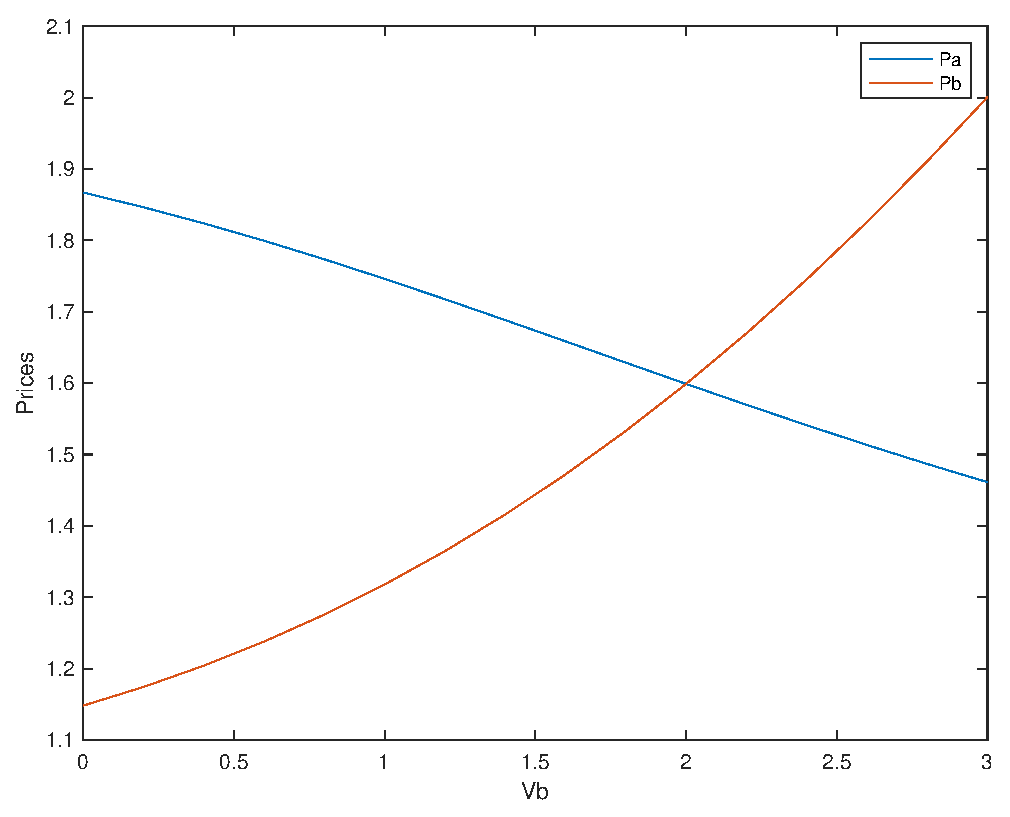
\includegraphics[width=\maxwidth{56.196688409433015em}]{figure_0}
\end{center}


\matlabheading{Question 4}

\begin{par}
\begin{flushleft}
Plot next period optimal stock (or harvest amount if you prefer) as a function of today's price for different amounts of lumber left in stock.
\end{flushleft}
\end{par}

\begin{matlabcode}
x25=policy(51,:);
x50=policy(101,:);
x75=policy(151,:);
x100=policy(201,:);

figure
plot(pgrid, x25, pgrid, x50, pgrid, x75, pgrid, x100);
title('Next period stock vs current price')
xlabel('price')
ylabel('Next period stock')
legend({'x=25', 'x=50', 'x=75', 'x=100'}, 'Location', 'best')
\end{matlabcode}
\begin{center}
\includegraphics[width=\maxwidth{56.196688409433015em}]{figure_1}
\end{center}


\matlabheading{Question 5}

\begin{par}
\begin{flushleft}
Assume firm starts with stock of 100 and todays price is 1. Plot expected stock over time for 20 periods ahead. Include the 90 percent confidence interval
\end{flushleft}
\end{par}

\begin{matlabcode}
P=zeros(nxgrid*npgrid, nxgrid*npgrid);

% Transition matrix for the states
for i=1:npgrid
    for j=1:npgrid
     P((i-1)*nxgrid+1:i*nxgrid, (j-1)*nxgrid+1:j*nxgrid)=prob(i,j)*(kron(ones(1,nxgrid), policy(:,i))==kron(ones(nxgrid,1),xgrid'));
    end
end

% For the following periods ahead
nperiods=20;

% Store distribution over states here
q=zeros(nperiods+1,nxgrid*npgrid);

% Start at p=1, x=100
q(1,11*nxgrid)=1;

for t=1:nperiods
 q(t+1,:)=q(t,:)*P;
end

% Expected Values

% Store the marginal probability distributions of x

x_margdist=zeros(nperiods+1, nxgrid);

for t=1:nperiods+1
    mat_q=reshape(q(t,:),[nxgrid,npgrid]);
    x_margdist(t,:)=sum(mat_q,2)';
end

% Expected values
mu_x=x_margdist*xgrid;

% Confidence interval
index=1:nxgrid;

% Cumulative distributions
x_cumsum=cumsum(x_margdist,2);

% Obtain 90th quantiles
indices90=zeros(nperiods+1,1);
for t=1:nperiods+1
    indices90(t,1)=min(index(x_cumsum(t,:)>=0.8));  
end
x90=xgrid(indices90);

lb=zeros(nperiods+1,1);
time=0:20;

plot(time, mu_x, time, x90, time, lb)

title('Expected Stock and 90% Confidence interval over time')
xlabel('time')
ylabel('stock')
legend({'Expected Stock', 'Upper bound for CI', 'Lower Bound for CI'}, 'Location', 'best')
\end{matlabcode}
\begin{center}
\includegraphics[width=\maxwidth{56.196688409433015em}]{figure_2}
\end{center}


\matlabheading{Question 6.}

\begin{par}
\begin{flushleft}
Redo 2-4 for the coarse grid of 5 points in Tauchen's representation
\end{flushleft}
\end{par}

\begin{par}
\begin{flushleft}
Question 6.2. Take a look at tauchen.m in the repository, use it to generate a grid that approximates the process for $p_t$ with 5 grid points
\end{flushleft}
\end{par}

\begin{matlabcode}

% Number of grid points for the price
npgrid=5;
[prob, pgrid, invdist]=tauchen(npgrid, cp_0, crho, sigma_u);

% Number of grid points for the stock of timber
nxgrid=201;

% Grid for timber stock
xgrid=linspace(0,100, nxgrid)';
\end{matlabcode}

\matlabheading{Question 6.3}

\begin{par}
\begin{flushleft}
Solve the firm's problem using value function iteration.  Plot the value of the firm depending on its initial stock (x-axis) and the current price of timber for $p\in\{ 0.9,1, 1.1\}$.
\end{flushleft}
\end{par}

\begin{matlabcode}
% Value function iteration
% Initial Value function matrix
Vold=zeros(nxgrid, npgrid);

% Store updated values here
Vnew=zeros(nxgrid, npgrid);

% Store policy indices here
pol_index=zeros(nxgrid, npgrid);

% Amount Harvested
h=xgrid-xgrid';

% Value function iteration

for j=1:npgrid
 values=period_profit(h,pgrid(j)) + cdelta*prob(j,:)*Vold';
 Vnew(:,j)=max(values,[],2);
end

diff=norm(Vnew-Vold)/norm(Vnew);

tol=0.00001;

iters=0;
while diff>tol
 Vold=Vnew;
 for j=1:npgrid
  values=period_profit(h,pgrid(j)) + cdelta*prob(j,:)*Vold';
  [Vnew(:,j), pol_index(:,j)]=max(values,[],2);
 end

 diff=norm(Vnew-Vold)/norm(Vnew);
 iters=iters+1;
end

policy=xgrid(pol_index);

% Plot the value of the firm
v0_9=Vnew(:,2);
v1=Vnew(:,3);
v1_1=Vnew(:,4);

figure
plot(xgrid, v0_9, xgrid, v1, xgrid, v1_1)
title('Value function vs Initial stock')
xlabel('stock')
ylabel('Value')
legend({'p~0.9', 'p~1.1', 'p~1.1'}, 'Location', 'best')
\end{matlabcode}
\begin{center}
\includegraphics[width=\maxwidth{56.196688409433015em}]{figure_3}
\end{center}


\matlabheading{Question 6.4}

\begin{par}
\begin{flushleft}
Plot next period optimal stock (or harvest amount if you prefer) as a function of today's price for different amounts of lumber left in stock.
\end{flushleft}
\end{par}

\begin{matlabcode}
x25=policy(51,:);
x50=policy(101,:);
x75=policy(151,:);
x100=policy(201,:);

figure
plot(pgrid, x25, pgrid, x50, pgrid, x75, pgrid, x100);
title('Next period stock vs current price')
xlabel('price')
ylabel('Next period stock')
legend({'x=25', 'x=50', 'x=75', 'x=100'}, 'Location', 'best')
\end{matlabcode}
\begin{center}
\includegraphics[width=\maxwidth{56.196688409433015em}]{figure_4}
\end{center}

\end{document}
